% =========================================================================
% MÓDULO 2: EVOLUCIÓN ARQUITECTÓNICA A1-A5 Y OPTUNA TPE (DIAPOSITIVAS 6 A 9)
% =========================================================================

% --- DIAPOSITIVA 6: EVOLUCIÓN ARQUITECTÓNICA EN TT2 (DE A0 A A5b Y A5) ---
\begin{frame}{Evoluci\'on Arquitect\'onica en TT2: De \texttt{A0} hasta \texttt{A5b} y \texttt{A5}}{Cuatro modificaciones estructurales acopladas sobre la l\'inea base de TT1 \cite{ronneberger2015unet,rodas_valencia_tpe_ecog}}
  \centering
  \scriptsize
  \renewcommand{\arraystretch}{1.18}
  \setlength{\tabcolsep}{4.5pt}
  \begin{tabularx}{\textwidth}{@{} l l l >{\raggedright\arraybackslash}X @{}}
    \toprule
    \rowcolor{ipnDark}
    \textcolor{white}{\textbf{Variante}} &
    \textcolor{white}{\textbf{Eje de Redise\~no}} &
    \textcolor{white}{\textbf{Operador / Configuraci\'on}} &
    \textcolor{white}{\textbf{Efecto T\'ecnico y Ganancia en CV (\'Epoca 50)}} \\
    \midrule
    \textbf{\texttt{A0} (Base TT1)} & Punto de partida & \texttt{BatchNorm1d}, \texttt{Dropout} $0.30$ & L\'inea base inicial de referencia ($\mathbf{0.5489}$). \\
    \rowcolor{rowLight}
    \textbf{\texttt{A1}} & Normalizaci\'on & \textbf{\texttt{LayerNorm}} por instante $t$ & Elimina dependencia de estad\'isticas de lote ($\mathbf{+0.0605}$). \\
    \textbf{\texttt{A2}} & Regularizaci\'on & \textbf{\texttt{Dropout}} $0.30 \rightarrow \mathbf{0.10}$ & Conserva detalles finos de la envolvente ($\mathbf{+0.0110}$ aislado). \\
    \rowcolor{rowLight}
    \textbf{\texttt{A3}} & Sobremuestreo aislado & \texttt{ConvTranspose1d} sin \texttt{A1/A2/A4} & Inestable por s\'i sola; cae a $0.5173$ ($\mathbf{-0.0316}$ vs.\ \texttt{A0}). \\
    \textbf{\texttt{A4}} & Fusi\'on en Decoder & \textbf{\texttt{Up} $\to$ \texttt{Concat(skip)} $\to$ \texttt{Conv}} & Filtra conjuntamente el mapa sobremuestreado y el \textit{skip}. \\
    \rowcolor{rowLight}
    \textbf{\texttt{A5b}} & Integraci\'on lineal & \texttt{A1} + \texttt{A2} + \texttt{A4} + \textbf{Interp.\ Lineal} & Sobremuestreo fijo libre de pesos ($\mathbf{0.6779}$, $+0.1290$). \\
    \rowcolor{rowHighlight}
    \textbf{\texttt{A5} (Propuesta)} & Integraci\'on completa & \texttt{A1} + \texttt{A2} + \texttt{A4} + \textbf{\texttt{ConvTranspose1d} DW} & Sobremuestreo aprendible por canal (\texttt{groups}$=C$, $-99.8\%$ params vs.\ densa; alcanza $\mathbf{0.6837}$, $\mathbf{+0.1349}$). \\
    \bottomrule
  \end{tabularx}
  \fuente{Creaci\'on propia, obtenida del repositorio GitHub \cite{rodas_valencia_tpe_ecog}.}

  \takeaway{La convoluci\'on transpuesta \textit{depthwise} (\texttt{groups}$=C$) en \texttt{A5} a\~nade solo $4C$ pesos por nivel ($2048$ vs.\ $1\,048\,576$ en el nivel $8f$), evitando la sobreparametrizaci\'on y logrando la mayor fidelidad al acoplarse con \texttt{LayerNorm} y el nuevo orden del Decoder \cite{rodas_valencia_tpe_ecog}.}
\end{frame}

% --- DIAPOSITIVA 7: ENTRENAMIENTO, FUNCIÓN DE PÉRDIDA Y PARADA TEMPRANA ---
\begin{frame}{Entrenamiento, Funci\'on de P\'erdida H\'ibrida y Parada Temprana}{Alineaci\'on simult\'anea de amplitud y fase temporal en trayectorias continuas \cite{wang2025dtcnet,loshchilov2019decoupled,rodas_valencia_tpe_ecog}}
  \begin{columns}[T,onlytextwidth]
    \begin{column}{0.49\textwidth}
      \begin{block}{1. Funci\'on de P\'erdida H\'ibrida Compuesta}
        \scriptsize
        Para evitar predicciones planas cercanas a la media, la funci\'on objetivo pondera en partes iguales el error de escala ($\operatorname{MSE}$) y la distancia coseno temporal ($\mathcal{L}_{\text{cos}}$) \cite{wang2025dtcnet,Sliwowski2022}:
        \[
          \mathcal{L}(\mathbf{Y}, \hat{\mathbf{Y}}) = 0.5\,\operatorname{MSE}(\mathbf{Y}, \hat{\mathbf{Y}}) + 0.5\big(1 - \operatorname{CosSim}_{\text{temp}}(\mathbf{Y}, \hat{\mathbf{Y}})\big)
        \]
        \begin{itemize}\setlength{\itemsep}{2pt}
          \item $\operatorname{MSE}$: Penaliza desviaciones de amplitud absoluta en $[0,1]$.
          \item $1 - \operatorname{CosSim}_{\text{temp}}$: Maximiza directamente la correlaci\'on morfol\'ogica y la sincron\'ia de fase de los picos de flexi\'on.
        \end{itemize}
      \end{block}
    \end{column}

    \begin{column}{0.47\textwidth}
      \begin{block}{2. Optimizador \texttt{Adam} con $L_2$ Acoplada}
        \scriptsize
        \begin{itemize}\setlength{\itemsep}{3pt}
          \item \textbf{Regla de actualizaci\'on:} \texttt{Adam} est\'andar con penalizaci\'on $L_2$ acoplada en el gradiente ($\tilde{g}_i = \nabla_{w_i}\mathcal{L} + \lambda w_i$) \cite{loshchilov2019decoupled}.
          \item \textbf{Estabilidad num\'erica:} Tama\~no de lote $B=128$ y recorte de norma global de gradiente $\|\mathbf{g}\|_2 \le 1.0$.
        \end{itemize}
      \end{block}

      \begin{alertblock}{3. Pol\'itica de \textit{Early Stopping}}
        \scriptsize
        Selecci\'on del mejor \textit{checkpoint} de validaci\'on bajo la regla:
        \[
          \text{min\_epochs} = 15, \quad \text{patience} = 10, \quad \text{max\_epochs} = 50
        \]
      \end{alertblock}
    \end{column}
  \end{columns}
\end{frame}

% --- DIAPOSITIVA 8: OPTIMIZACIÓN BAYESIANA MEDIANTE OPTUNA TPE ---
\begin{frame}{Optimizaci\'on Bayesiana mediante Optuna TPE}{B\'usqueda conjunta de arquitectura e hiperpar\'ametros adaptada por sujeto \cite{Bergstra2011,akiba2019optuna,rodas_valencia_tpe_ecog}}
  \begin{columns}[T,onlytextwidth]
    \begin{column}{0.47\textwidth}
      \begin{block}{Muestreador TPE en Optuna}
        \scriptsize
        \begin{itemize}\setlength{\itemsep}{3pt}
          \item El estimador \textit{Tree-structured Parzen Estimator} (TPE) modela dos densidades sobre el historial ($\gamma = 0.25$) \cite{Bergstra2011,akiba2019optuna}:
            \begin{itemize}\scriptsize
              \item $\ell(\bm{\lambda})$: Configuraciones en el cuartil superior.
              \item $g(\bm{\lambda})$: Configuraciones restantes.
            \end{itemize}
          \item Maximiza la mejora esperada seleccionando candidatos que maximizan el cociente $\ell(\bm{\lambda}) / g(\bm{\lambda})$.
          \item \textbf{Funci\'on objetivo por sujeto $s$:}
            \[
              J(\bm{\lambda}, s) = \frac{1}{5}\sum_{k=1}^{5}\left[\max_{e \in E_{s,k,\bm{\lambda}}} r_{s,k,e}^{\text{val}}\right]
            \]
        \end{itemize}
      \end{block}
    \end{column}

    \begin{column}{0.49\textwidth}
      \begin{block}{Espacio de B\'usqueda Mixto ($\Lambda$) y Presupuesto}
        \scriptsize
        \centering
        \renewcommand{\arraystretch}{1.2}
        \setlength{\tabcolsep}{2.8pt}
        \begin{tabular}{@{} l l l @{}}
          \toprule
          \rowcolor{ipnDark}
          \textcolor{white}{\textbf{Hiperpar\'ametro}} &
          \textcolor{white}{\textbf{Escala}} &
          \textcolor{white}{\textbf{Dominio Explorado}} \\
          \midrule
          \texttt{architecture\_id} & Categ\'orica & $\{\texttt{A5},\; \texttt{A5b}\}$ \\
          \rowcolor{rowLight}
          Learning rate ($\eta$) & Log-continua & $[5\times 10^{-5},\; 5\times 10^{-4}]$ \\
          Regularizaci\'on $L_2$ ($\lambda$) & Log-continua & $[10^{-7},\; 10^{-3}]$ \\
          \rowcolor{rowLight}
          Tama\~no de kernel ($k$) & Categ\'orica & $\{5,\; 7\}$ \\
          Niveles U-Net ($L$) & Entera & $\{4,\; 5\}$ \\
          \rowcolor{rowLight}
          Canales base ($f$) & Categ\'orica & $\{64,\; 96\}$ \\
          \bottomrule
        \end{tabular}
        \fuente{Creaci\'on propia, obtenida del repositorio GitHub \cite{rodas_valencia_tpe_ecog}.}
        \vspace{1mm}

        {\scriptsize\textbf{Presupuesto 100\% completado:} $32\text{ trials/sujeto}$ ($10$ \textit{warmups} balanceados $5\text{ \texttt{A5}}/5\text{ \texttt{A5b}} + 22\text{ TPE}$) $\times 5\text{ folds} = \mathbf{480\text{ entrenamientos}}$.}
      \end{block}
    \end{column}
  \end{columns}
\end{frame}

% --- DIAPOSITIVA 9: DINÁMICA DE EXPLORACIÓN EN OPTUNA TPE ---
\begin{frame}{Din\'amica de Exploraci\'on y Capacidad en Optuna TPE}{Evoluci\'on de los 32 ensayos por sujeto y relaci\'on entre n\'umero de par\'ametros y objetivo CV \cite{akiba2019optuna,rodas_valencia_tpe_ecog}}
  \begin{columns}[T,onlytextwidth]
    \begin{column}{0.48\textwidth}
      \centering
      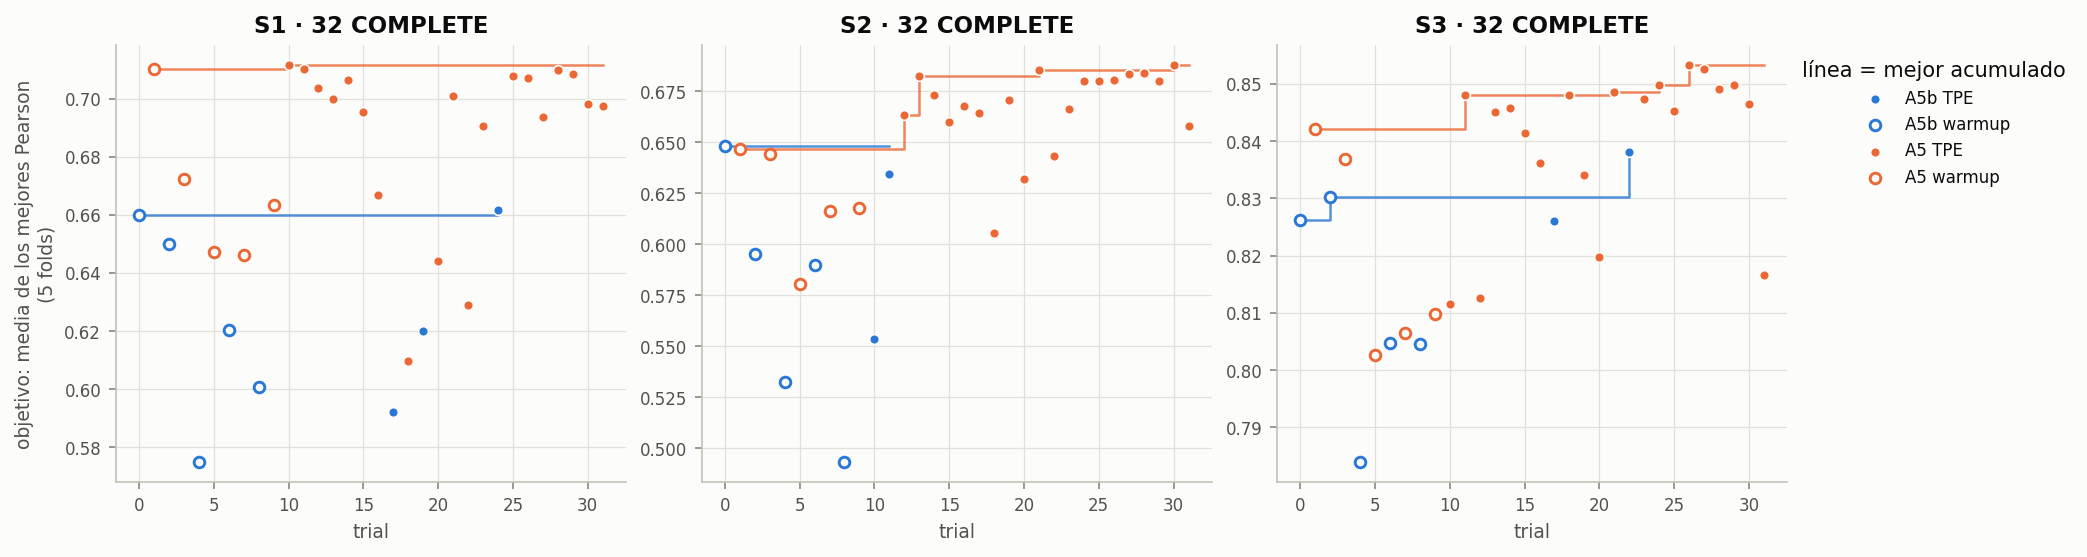
\includegraphics[width=\linewidth,height=0.47\textheight,keepaspectratio]{imgs/optimization_history.png}
      \figcap{2}{Historial de optimizaci\'on a lo largo de los $32$ ensayos por sujeto ($96$ trials totales) en Optuna TPE. \textbf{Fuente:} Obtenida del repositorio GitHub \cite{rodas_valencia_tpe_ecog}.}
    \end{column}
    \begin{column}{0.48\textwidth}
      \centering
      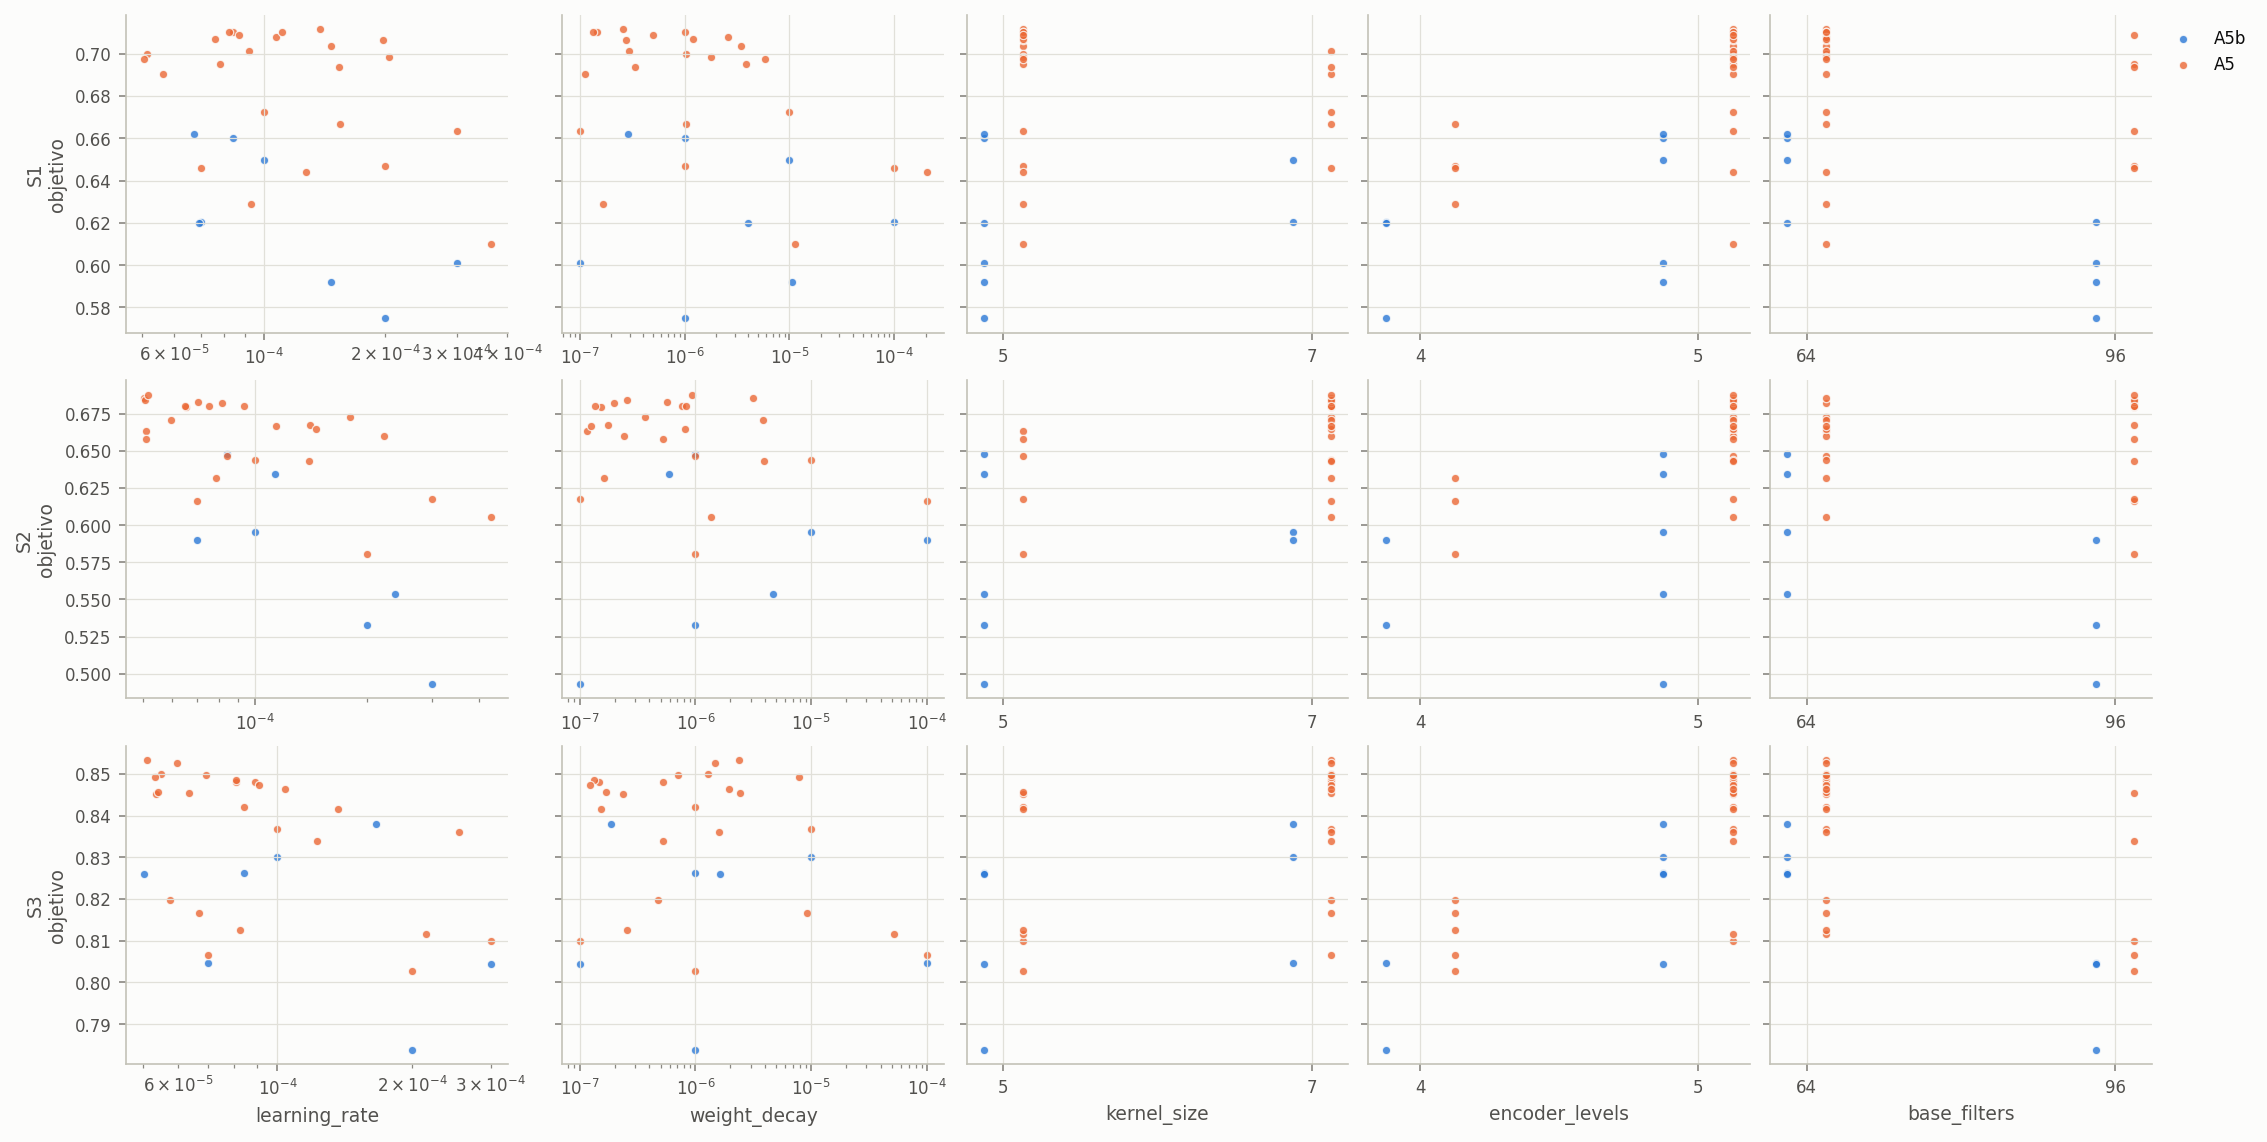
\includegraphics[width=\linewidth,height=0.47\textheight,keepaspectratio]{imgs/params_vs_objective.png}
      \figcap{3}{Relaci\'on entre complejidad param\'etrica ($N_{\text{params}}$), familia arquitect\'onica (\texttt{A5} vs.\ \texttt{A5b}) y correlaci\'on CV. \textbf{Fuente:} Obtenida del repositorio GitHub \cite{rodas_valencia_tpe_ecog}.}
    \end{column}
  \end{columns}

  \takeaway{En \texttt{S1} y \texttt{S3} las redes moderadas ($f=64$, $9.35\text{--}12.71\text{ M}$ params) saturan tempranamente el techo de validaci\'on, mientras que en el paciente m\'as complejo (\textbf{\texttt{S2}}) TPE identifica una mejora clara al escalar hacia mayor capacidad representacional ($k=7, L=5, f=96$, $28.03\text{ M}$ params) \cite{rodas_valencia_tpe_ecog}.}
\end{frame}
